%!TEX root = ../NCVC.tex

\mysection{基本編}

\subsection{CADでの作図}

\begin{minipage}[t]{0.4\textwidth}
 まずは基本的な加工を行うための基本的な作図方法を解説します.
図\ref{fig:sample1.jww} のような図形を書きましょう.
切削対象(ワーク)を示す矩形と,その矩形左下に円を1つ.
「NCVC」という文字は,線をつなぎ合わせたデータです.
\end{minipage}
\begin{minipage}[t]{0.6\textwidth}
\vspace*{-2zh}
\begin{figure}[H]
\centering
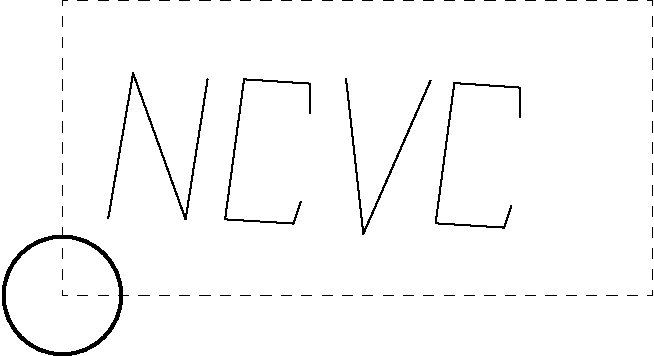
\includegraphics[scale=0.8]{No1/fig/sample1.pdf}
\caption{サンプル図形}
\label{fig:sample1.jww}
\end{figure}
\end{minipage}

\vspace*{2zh}
 NCVCはCADでの作図情報を全て読み込むのではなく,
特定のレイヤ情報を元に作図データを読み込みます.
CADでの作図において必要とされる補助線や寸法線等が加工データには必要なく,
これらを選別するための仕様です.

 その選別方法は『必要なレイヤに名前を付ける』こと.
図\ref{fig:sampleLayer.png} は図\ref{fig:sample1.jww} のレイヤ情報ですが,
0番レイヤに「ORIGIN」という名前,
1番レイヤに「CAM\_LINE」という名前を付けています.
それぞれ機械原点と切削軌跡を示し,この2つのレイヤは必須です
\footnote{実は機械原点レイヤは必須ではありません.詳細は【穴加工】の節で解説しています.}.
機械原点レイヤには工作機械のXY原点を示す円を1つだけ作図.
大きさは任意ですが,円の中心がXYの原点となります.
切削軌跡 CAM\_LINE レイヤには刃物のパス,
すなわち削りたい図形を書きます.
他,ワーク矩形を示す補助線等は別のレイヤに書きます.
レイヤに名前を付ける方法は,それぞれのCAD操作に準拠して下さい.
なお,全てのデータにおいて線種,線色は関係ありません.

\vspace*{1zh}
\begin{figure}[H]
\centering
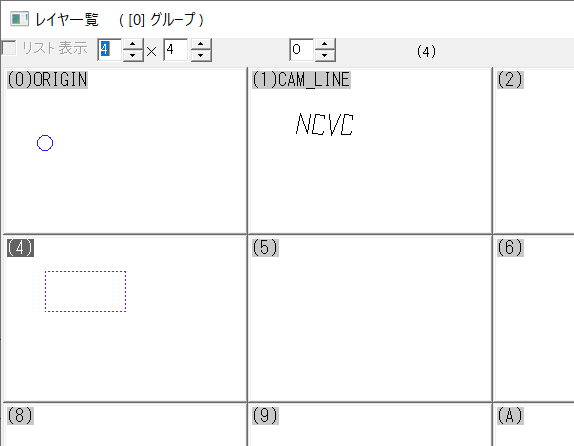
\includegraphics{No1/fig/sampleLayer.png}
\caption{レイヤ一覧}
\label{fig:sampleLayer.png}
\end{figure}

 作図が終わればCADデータをDXF形式で保存します
\footnote{
    Jw\_cadの場合,DXF形式で保存する必要はありません.NCVCはJWW形式を直接読み込むことが可能です.
    詳細は【パワーユーザ編】の【アドイン作成のすすめ】を参照して下さい.
}.
NCVCにCADデータを読み込ませるためDXF形式で保存する必要がありますが,
多くの場合,DXF形式で保存するとそのCAD独自のデータが失われるため,
使用しているCAD独自の形式でも保存しておきましょう.

\subsection{CADデータの読み込み}

\begin{minipage}[t]{0.5\textwidth}
 NCVCでDXF形式のCADデータを読み込みます.
が,その前に確認.
NCVCの \menu{オプション>DXF関連の設定} をクリックし,
NCVCが読み込むレイヤ名を設定して下さい.
デフォルトで先ほど設定した値になっていると思います.
基本編では[従来互換]のみ解説しますので,図\ref{fig:NCVCsetup.png} の通り設定して下さい.
この値は任意です.CAD側の設定と合わせて下さい.
無事読み込めると原点を示す十字(大きさは原点円の直径)と切削対象のパスが表示されます.
原点レイヤと切削レイヤ以外に作図した情報,
例えば,図\ref{fig:sampleLayer.png} の4番レイヤに書いたワークを表す矩形は読み込まれません(図\ref{fig:NCVCread.png}).
CADでの線種・線色は無視され,NCVCの設定に基づき表示されます.
詳細はリファレンスの表示属性を参照してください.
\end{minipage}
\begin{minipage}[t]{0.5\textwidth}
\vspace*{-2zh}
\begin{figure}[H]
\centering
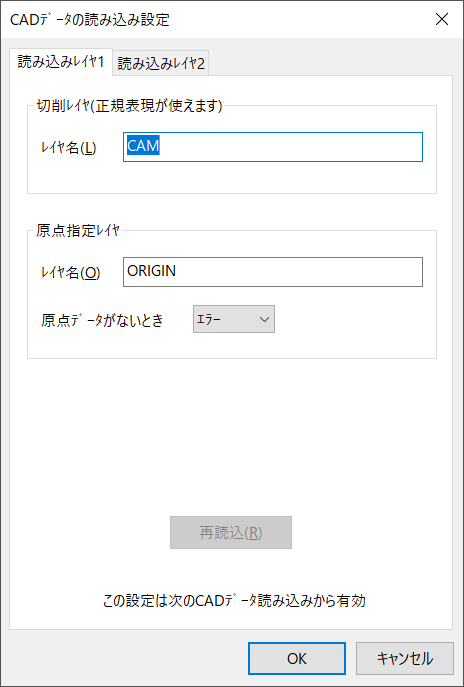
\includegraphics[scale=0.8]{No1/fig/NCVCsetup.png}
\caption{読み込みレイヤ設定}
\label{fig:NCVCsetup.png}
\end{figure}
\end{minipage}

\begin{figure}[H]
\centering
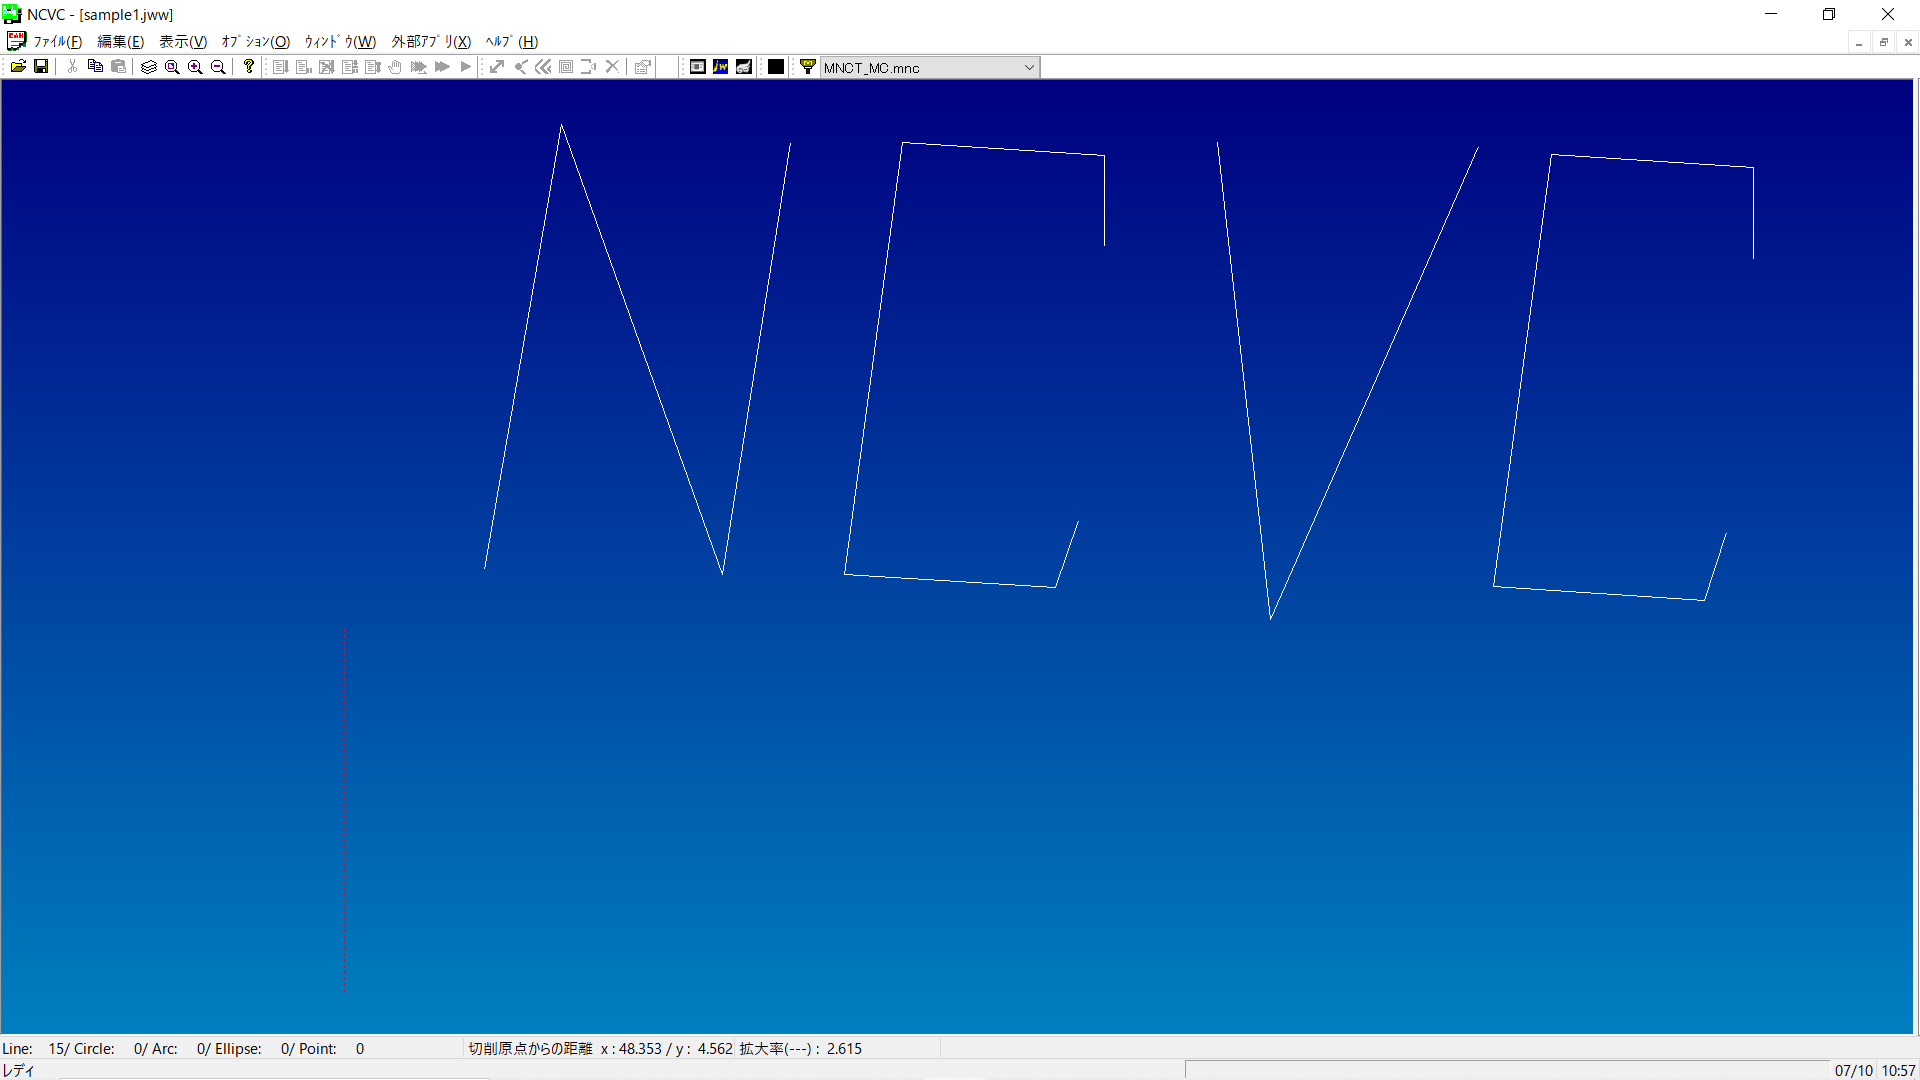
\includegraphics[scale=0.4]{No1/fig/NCVCread.png}
\caption{CADデータの読み込み}
\label{fig:NCVCread.png}
\end{figure}
